% !TEX root =  ../main.tex
\section{MaxSpareResources}

\subsection{Definition}

\subsubsection{Signature} \cstr{maxSpareResources(s : set<server>, rc : string, n : number)}

\begin{itemize}
\item \cstr{s} : a non-empty set of servers for a meaningful constraint.
\item \cstr{rc} : a resource identifier such as \cstr{mem}, \cstr{ucpu}, \cstr{pcpu} or \cstr{nodes} to identify the physical memory,
the computational capacity, the physical CPUs or the node itself, respectively.
\item \cstr{n} : a positive number
\end{itemize}

The \cstr{maxSpareResources} restricts to at most \cstr{n}, the number of free resources directly
available for VMs on the online servers in \cstr{s}. Servers in the \st{Offline} state are ignored.


\classification{maxSpareResources}{datacenter administrator}{Resource allocation}{Resource management,Power saving,Capacity planning}

\subsubsection{Usage}

This constraint deserves a power saving concern. 
The most effective solution to reduce the energy consumption of a non-saturated datacenter is to turn off unused servers and to turn on and off servers depending on the load variation.
When a load spike arise, it may then be a necessary to put some servers online to make their resources available to the VMs.~\cite{hermenier-xhpc06,vmware-dpm}
The time to boot the awaited servers may however be significant and alter the reactivity of the datacenter
when it faces an emergency situations. One solution is to let online a controlled number
of \emph{spare} resources that can be used instantly to absorb the load increase.
A datacenter administrator may then use one \cstr{maxSpareResources} constraint
to control the maximum number of unused servers to let online while the others will
be turned off to save power.

It is worth noting that despite this constraint is applicable to a various number of resources, it is preferable to only focus
the \cstr{nodes} resource. Indeed, a server provides resources at a coarse grain and it may not be possible to manage the resources according to the constraint by only managing the servers state.

\subsubsection{Example}

Figure~\ref{fig: maxSpareResources} depicts a sample reconfiguration between a source and a destination configuration where each server provides 8 unit of CPU and 7 unit of memory resources to VMs. During the reconfiguration, several relocations have been performed and the server \cstr{N3} has been turned off to save power. In this setting, the following \cstr{maxSpareResources} constraints were considered:

\begin{figure}[htb]
\centering
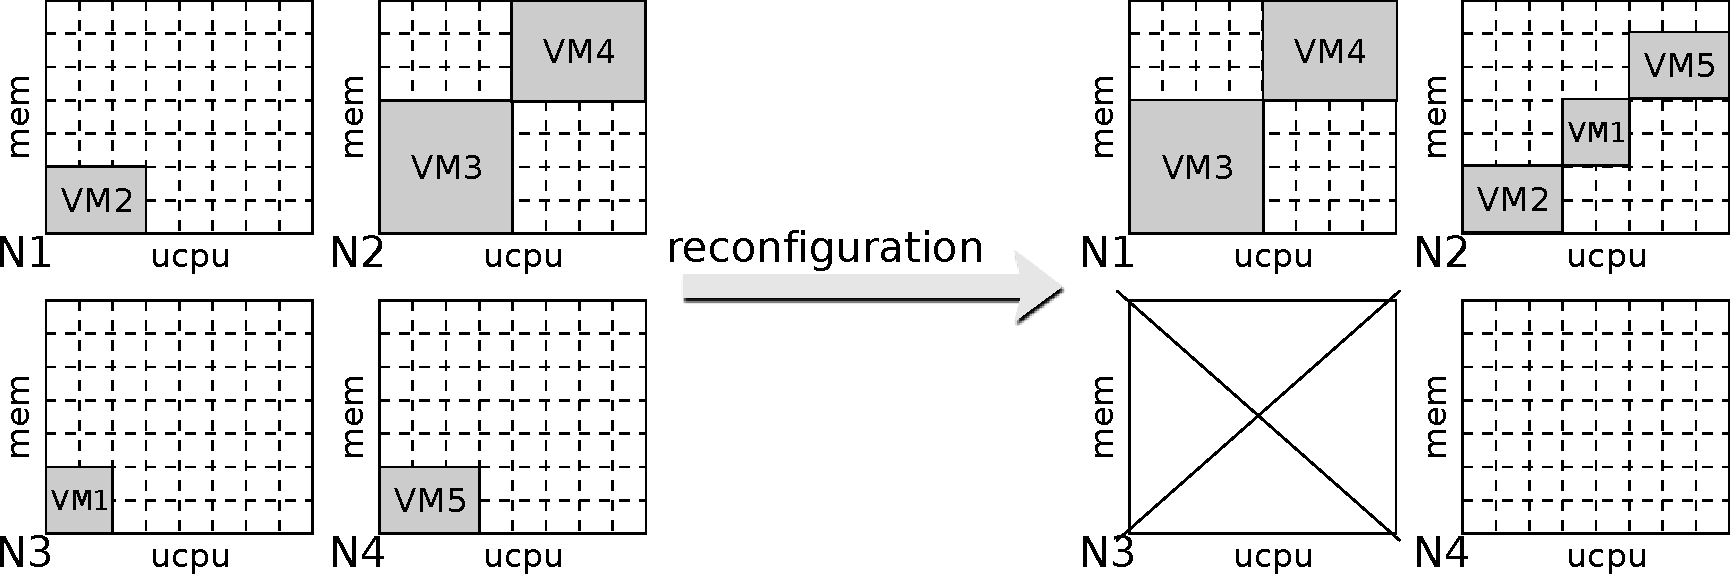
\includegraphics[width=\textwidth]{img/maxSpareResources}
\caption{A reconfiguration motivated by \cstr{maxSpareResources} constraints.}\label{fig: maxSpareResources}
\end{figure}


\begin{itemize}

\item \cstr{maxSpareResources(\{N2,N3,N4\},"node",1)}. This constraint was satisfied in the source configuration as no server was idle. The constraint is still satisfied in the destination configuration as only \cstr{N4} is in the \st{Online} state and idle.

\item \cstr{maxSpareResources(\{N1,N2,N3\},"ucpu",10)}. This constraint was not satisfied in the source configuration
as 11 uCPU was directly available to the running VMs. The reconfiguration fixed this violation. With the shutdown of \cstr{N3},
8 uCPU resources are directly available in the destination configuration, which is an amount allowed by the constraint.

\item \cstr{maxSpareResources(\{N1, N3\},"mem",3)}. This constraint was not satisfied in the source configuration
as 10 unit of memory were directly available to the running VMs. The reconfiguration fixed this violation. With the shutdown of \cstr{N3}, and the saturation of \cstr{N1}, no memory resources are left available to the VMs on these servers.

\end{itemize}

\fullVersion{
\subsection{Model}

The \cstr{noIdleOnlines} constraint is modeled in terms of the RPs variable by restricting
the state variable of each involved server to 0 depending on the number of VMs running
on the servers.

\begin{equation*}
\begin{split}
\forall N \in \mathcal{N},\ offline(N) & \triangleq\\
&	\forall n_i \in N, 
\sum_{d_i |�v_i \in \mathcal{V}} d_i = 0 \imply n_i^q = 0
\end{split}
\end{equation*}

\subsection{Violation detection}

To compute the list of violating elements, it is a necessary to check for each of 
the involved  server that are still online without running any VMs. This indicates
the violating servers.


\subsection{Availability}

\subsubsection{In {\btrp}}

The constraint is available in {\btrp} under the name \cstr{noIdleOnlines}.
To check whether a server is running a VM or not, we rely on the variable
indicating its memory usage. When this variable equals 0, then it is considered
the server does not host any VM and has to be turned off.

\begin{equation*}
\begin{split}
\forall N \in \mathcal{N},\ offline(N) & \triangleq\\
&	\forall n_i \in N,  eq(n_i^{mem}, 0) \imply eq(n_i^q, 0)
\end{split}
\end{equation*}
}

\subsection{See also}

\subsubsection{Related Constraints}
\begin{itemize}
\item \cstrref{minSpareResources}: This constraint restricts the number of unused online servers to a given minimum.
\end{itemize}

\printListOfInheritance{maxSpareResources}
%
%\begin{itemize}
%\item \hyperref[cstr: offline]{\cstr{offline}}: The turn off servers in any condition.
%\end{itemize}